\chapter{Phân tích và trực quan hóa dữ liệu}\label{ch:phantich}\label{ch:trucquan}

Chương này trình bày bảy phép phân tích trên dữ liệu đã làm sạch (13,580 dòng) cùng năm biểu đồ thuộc năm dạng khác nhau, chỉ giữ các kết quả phục vụ phần mô hình. Mỗi phép gồm mục đích, phương pháp, kết quả và diễn giải. Các bảng \texttt{price\_*}, \texttt{top\_suburbs}, \texttt{price\_distance\_corr} và các biểu đồ \texttt{01\_*.png} đến \texttt{05\_*.png} do \texttt{pipeline.py} ghi vào \texttt{outputs/}; các số còn lại do \texttt{build\_report\_metrics()} ghi vào \texttt{outputs/report\_metrics.csv}, truy theo mã. Giá tính bằng đô la Úc (AUD), là giá danh nghĩa. \label{sec:nguyentac}\label{sec:bieudo}\label{sec:groupby}Mỗi biểu đồ có tiêu đề, nhãn trục và đơn vị; dạng biểu đồ chọn theo bản chất dữ liệu, và giá tổng hợp theo nhóm bằng trung vị vì giá lệch phải.

\section{Phân phối của giá}\label{sec:mota}\label{sec:p1}
\paragraph{Mục đích và phương pháp.} Xác định giá lệch đến mức nào để chọn cách biểu diễn khi mô hình hóa; dùng \texttt{describe()}, phân vị, độ lệch (\texttt{skew}) và hệ số biến thiên.
\paragraph{Kết quả.} Giá trung bình 1,075,684, trung vị 903,000, nhỏ nhất 85,000, lớn nhất 9,000,000; độ lệch 2.24 và còn 0.18 khi lấy logarit; hệ số biến thiên 0.59 (\texttt{outputs/price\_summary.csv}; \bs{L04, P01}).

\begin{figure}[H]
\centering
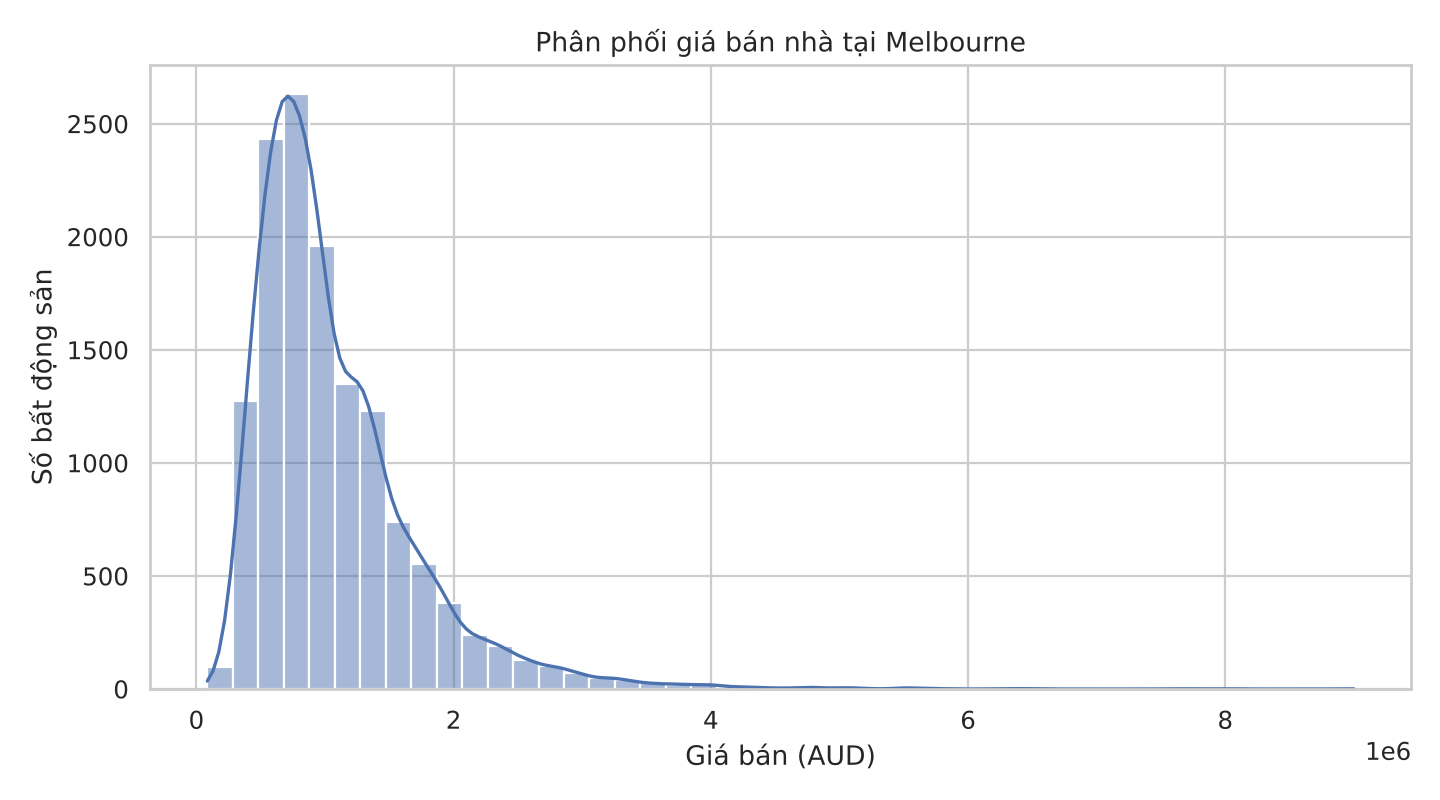
\includegraphics[width=0.72\linewidth]{01_price_distribution.png}
\caption{Phân phối giá bán nhà (histogram 45 khoảng kèm đường mật độ)}\label{fig:hist}
\nguon{\texttt{outputs/01\_price\_distribution.png}; số liệu kèm theo: \bs{P09}.}
\end{figure}

\paragraph{Diễn giải.} Trung bình cao hơn trung vị 19\% và đuôi phải kéo dài đến 9 triệu cho thấy phân phối lệch phải; 92.2\% giao dịch dưới 2 triệu (\bs{P09}). Vì vậy báo cáo dùng trung vị để so sánh nhóm, và logarit giá làm biến mục tiêu của Random Forest (mục~\ref{sec:ttr}). Trước khi loại ngoại lai, \texttt{Landsize} trung bình là 558.4 m\textsuperscript{2} (lớn nhất 433,014), sau khi loại là 478.3 trong khi trung vị gần như không đổi (440 và 439) (\bs{P02}).

\section{Giá theo nhóm (\texttt{groupby})}\label{sec:p2}\label{sec:p3}\label{sec:p4}\label{sec:p5}
Bốn phép dưới đây nhóm bằng \texttt{groupby}, lọc bằng \texttt{query} và sắp xếp bằng \texttt{sort\_values} trong \texttt{pipeline.py}.

\paragraph{Phép 2. Loại nhà.} Nhóm theo \texttt{Type}. Trung vị nhà riêng 1,080,000, liền kề 846,750, căn hộ 560,000, tức nhà riêng gấp 1.93 lần căn hộ và phân tán nhất (hệ số biến thiên 0.54 so với 0.42 và 0.43) (Bảng~\ref{tab:loainha}, Hình~\ref{fig:typebox}). Căn hộ nhỏ hơn (diện tích xây trung vị 75 m\textsuperscript{2} so với 144 m\textsuperscript{2}) và gần trung tâm hơn (6.9 km so với 10.4 km) (\bs{P03}), điều cần nhớ khi đọc tác động của khoảng cách ở Phép 6.

\begin{table}[H]
\centering
\caption{Giá theo loại nhà (AUD)}\label{tab:loainha}
\small
\begin{tabular}{@{}l r r r r r@{}}
\toprule
Loại nhà & Số giao dịch & Tỷ lệ & Trung vị & Trung bình & Hệ số biến thiên \\
\midrule
Nhà riêng (\texttt{h}) & 9,449 & 69.6\% & 1,080,000 & 1,242,665 & 0.54 \\
Liền kề (\texttt{t}) & 1,114 & 8.2\% & 846,750 & 933,735 & 0.42 \\
Căn hộ (\texttt{u}) & 3,017 & 22.2\% & 560,000 & 605,127 & 0.43 \\
\bottomrule
\end{tabular}
\nguon{\texttt{outputs/price\_by\_type.csv}; tỷ lệ: \bs{N09}; hệ số biến thiên: \bs{P03}.}
\end{table}

\begin{figure}[H]
\centering
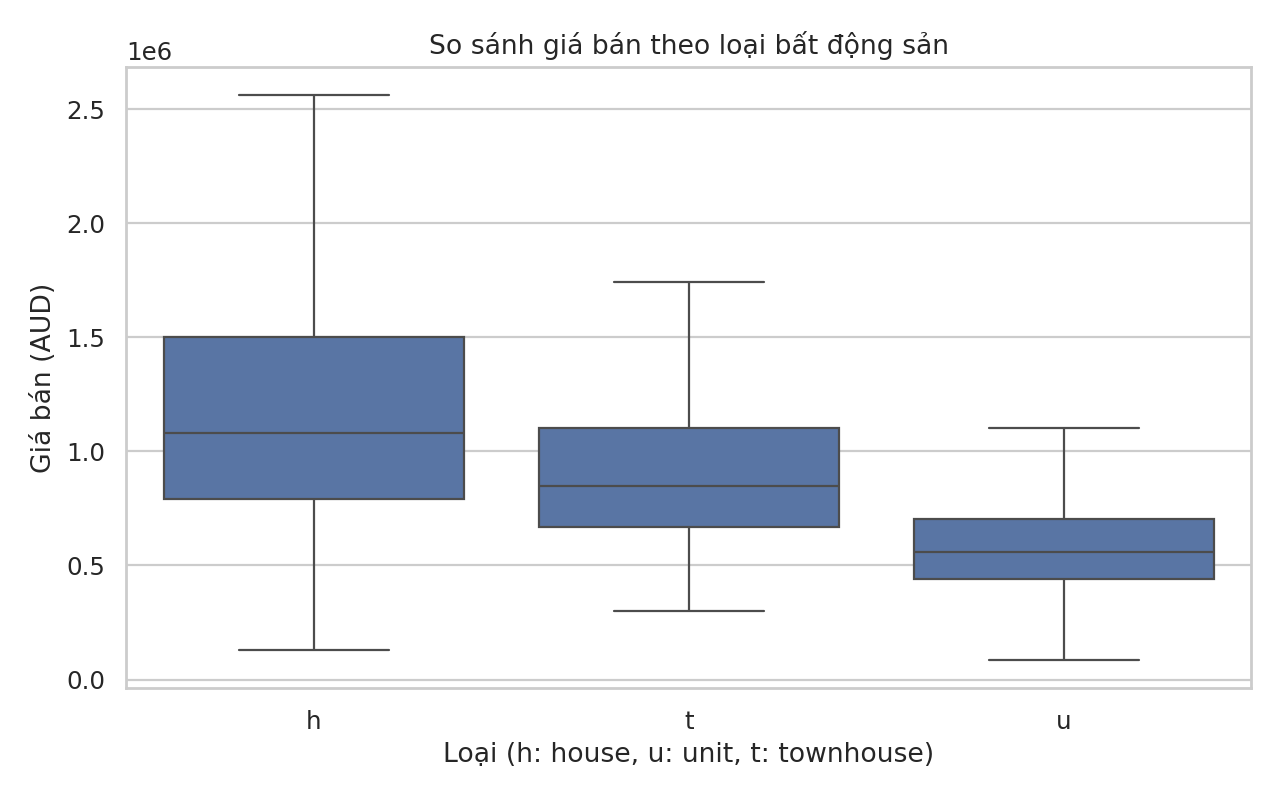
\includegraphics[width=0.72\linewidth]{02_price_by_type_boxplot.png}
\caption{Phân phối giá theo loại nhà (\texttt{h}: nhà riêng, \texttt{t}: liền kề, \texttt{u}: căn hộ)}\label{fig:typebox}
\nguon{\texttt{outputs/02\_price\_by\_type\_boxplot.png}; số liệu: \texttt{outputs/price\_by\_type.csv}.}
\end{figure}

\paragraph{Phép 3. Vùng.} Nhóm theo \texttt{Regionname} (8 vùng). Southern Metropolitan đắt nhất (trung vị 1,250,000), gấp 1.6 lần Western Metropolitan (793,000) (\bs{P04}; Hình~\ref{fig:region}). Ba vùng Victoria chỉ có 32 đến 53 giao dịch mỗi vùng nên kém tin cậy, và chênh lệch giữa các vùng còn lẫn với cơ cấu loại nhà.

\begin{figure}[H]
\centering
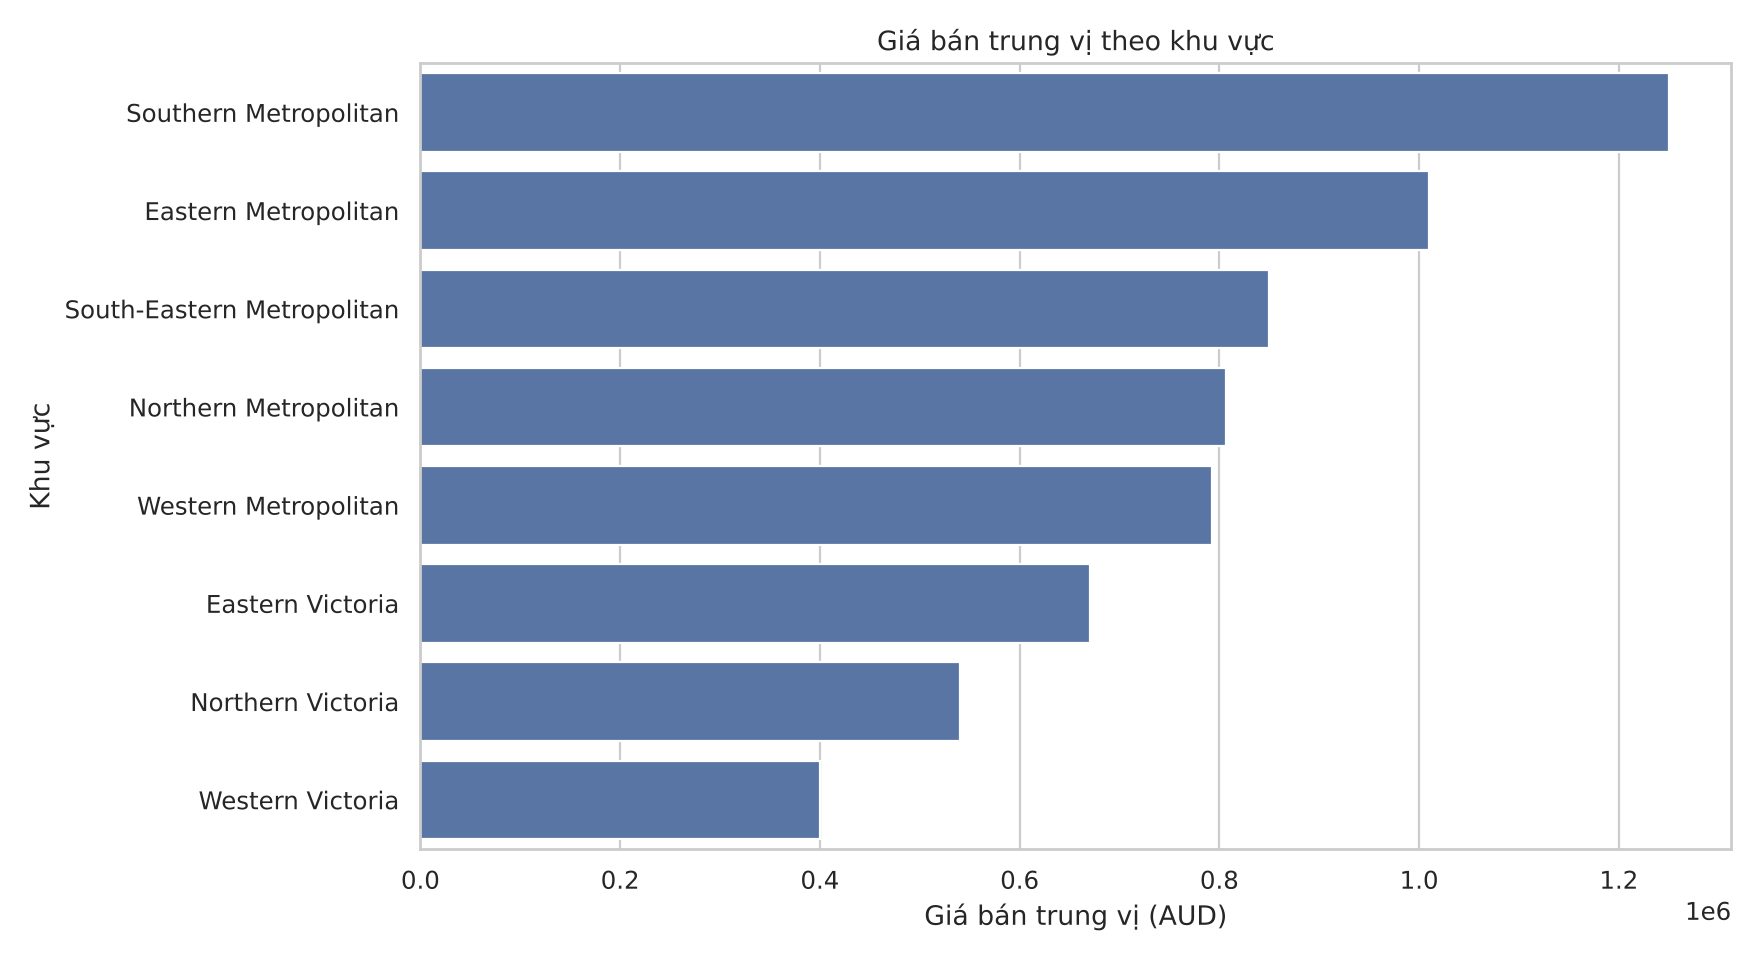
\includegraphics[width=0.72\linewidth]{03_median_price_by_region.png}
\caption{Giá trung vị theo vùng, sắp xếp giảm dần}\label{fig:region}
\nguon{\texttt{outputs/03\_median\_price\_by\_region.png}; số liệu: \texttt{outputs/price\_by\_region.csv}.}
\end{figure}

\paragraph{Phép 4. Số phòng.} Nhóm theo \texttt{Rooms}, giữ nhóm từ 20 giao dịch. Trung vị tăng từ 385,000 (1 phòng, 681 giao dịch) lên 690,000, 950,000, 1,285,000 và 1,660,000 (5 phòng); nhà 4 phòng đắt gấp 3.3 lần nhà 1 phòng, nhưng mức tăng thêm mỗi phòng giảm dần (+79\%, +38\%, +35\%, +29\%) (\bs{P05}; \texttt{outputs/price\_by\_rooms.csv}).

\paragraph{Phép 5. Suburb.} Nhóm theo \texttt{Suburb}, giữ suburb từ 30 giao dịch (125 trong 314 suburb; \bs{P06}) vì trung vị của suburb ít giao dịch dao động mạnh. Đứng đầu là Albert Park (1,900,000; 69 giao dịch), Canterbury (1,890,000), Middle Park (1,880,000), Balwyn (1,850,000) và Brighton (1,773,500), Albert Park gấp 2.1 lần trung vị chung (\texttt{outputs/top\_suburbs.csv}). Mô hình mã hóa suburb bằng one-hot (314 giá trị) nên các suburb thưa dữ liệu được học kém (mục~\ref{sec:hanche}).

\section{Tương quan với giá}\label{sec:tuongquan}\label{sec:p6}
\paragraph{Mục đích và phương pháp.} Xác định thuộc tính số liên hệ mạnh nhất với giá và kiểm tra ngoại lai về diện tích có làm sai lệch kết quả không: tính Pearson bằng \texttt{df[cols].corr()} và Spearman (\texttt{method="spearman"}), rồi so Pearson trước và sau khi loại ngoại lai (\texttt{build\_report\_metrics()}; ``trước khi loại'' là \texttt{data/melb\_data.csv} với \texttt{BuildingArea} $\leq$ 0 đặt thành thiếu).

\begin{figure}[H]
\centering
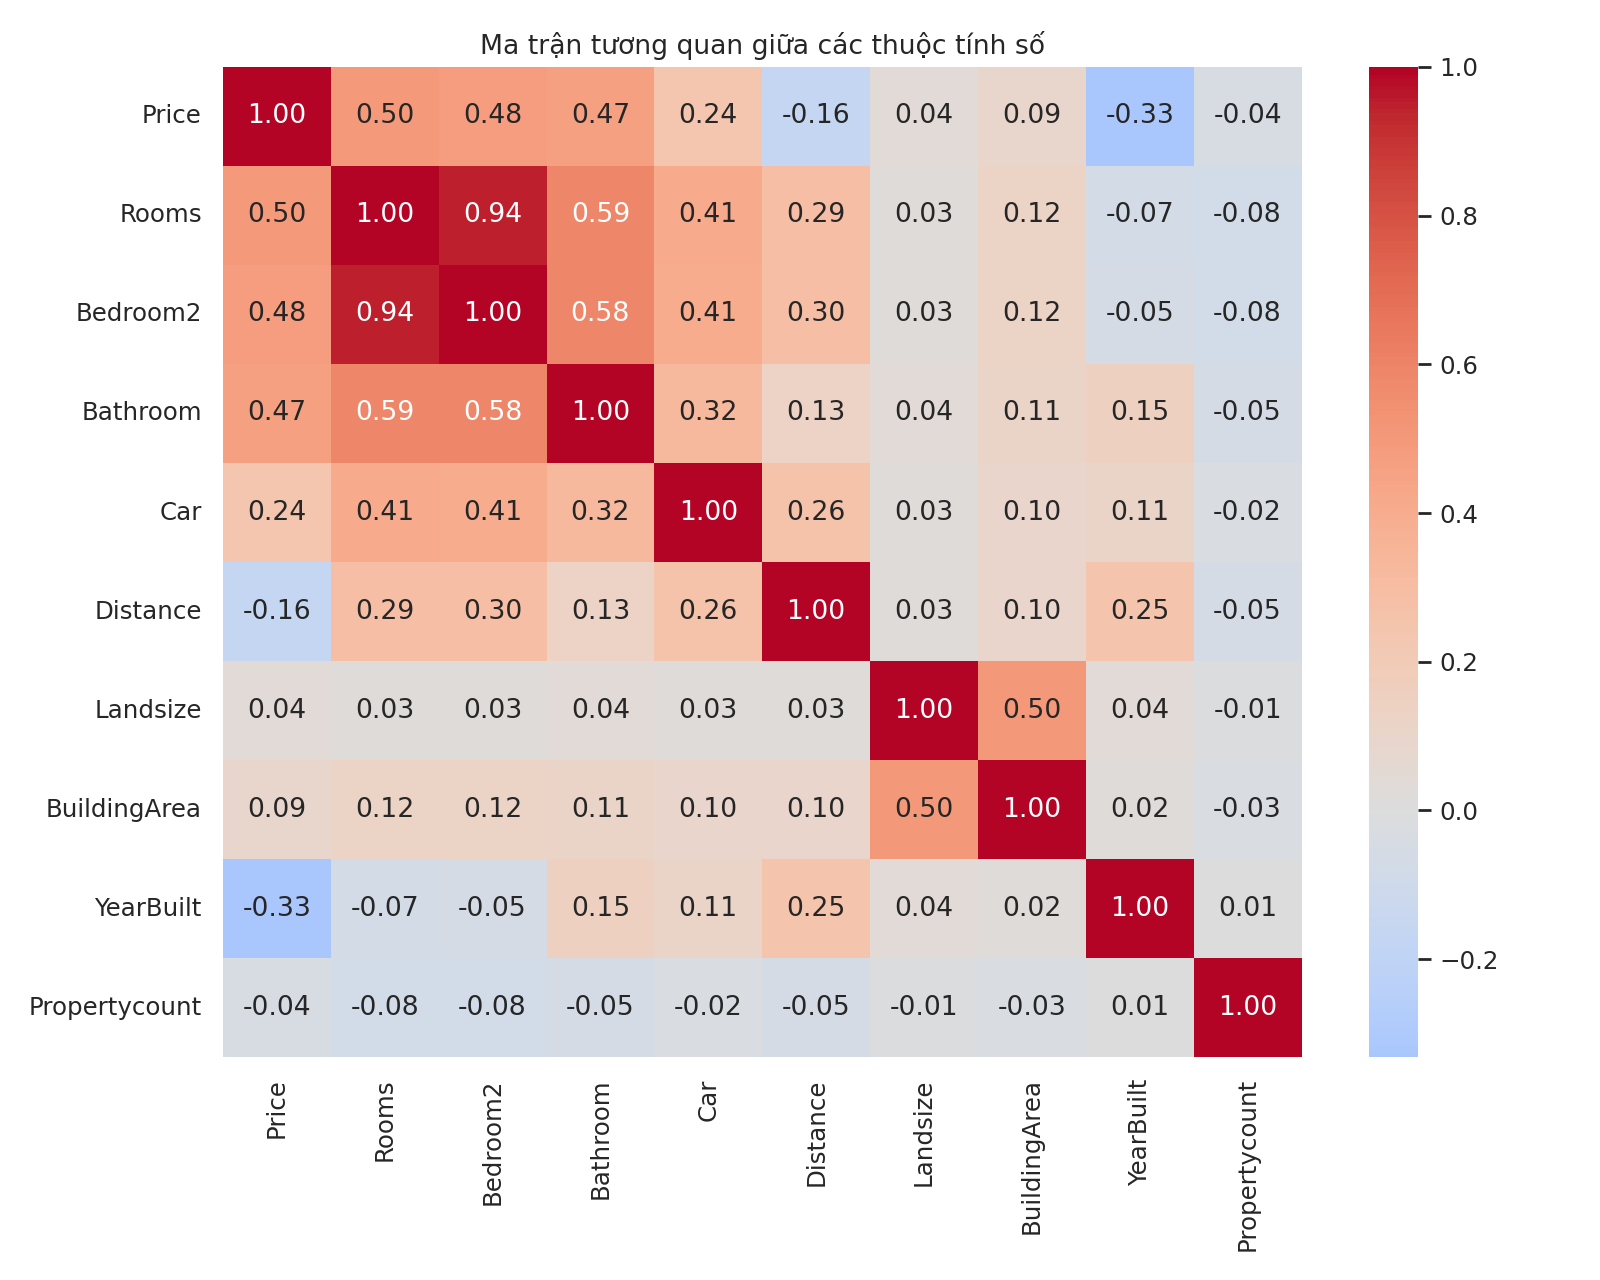
\includegraphics[width=0.8\linewidth]{05_correlation_heatmap.png}
\caption{Ma trận tương quan Pearson giữa giá và các thuộc tính số}\label{fig:corr}
\nguon{\texttt{outputs/05\_correlation\_heatmap.png}; giá trị: \bs{P07}.}
\end{figure}

\begin{table}[H]
\centering
\caption{Tương quan Pearson với giá trước và sau khi loại ngoại lai về diện tích}\label{tab:nhay}
\small
\begin{tabular}{@{}L{6.0cm} r r L{3.6cm}@{}}
\toprule
Thuộc tính & Trước & Sau & Spearman (sau) \\
\midrule
\texttt{BuildingArea} (loại 8 dòng $>$ 1,000 m\textsuperscript{2}) & 0.092 & 0.556 & 0.637 \\
\texttt{Landsize} (loại 26 dòng $>$ 10,000 m\textsuperscript{2}) & 0.038 & 0.132 & 0.329 \\
\bottomrule
\end{tabular}
\nguon{\bs{P07}; \texttt{outputs/price\_distance\_corr.csv} (một phần).}
\end{table}

\paragraph{Diễn giải.}
\begin{itemize}[nosep]
  \item Liên hệ mạnh nhất với giá: \texttt{BuildingArea} (0.556), \texttt{Rooms} (0.497), \texttt{Bedroom2} (0.476), \texttt{Bathroom} (0.469); \texttt{YearBuilt} ($-$0.332) và \texttt{Distance} ($-$0.163) tương quan âm. \texttt{Bedroom2} và \texttt{Rooms} gần như cùng một thông tin (0.944) (\bs{N06, P07}).
  \item Ngoại lai làm hệ số bị đánh giá thấp: tám dòng trên 1,000 m\textsuperscript{2} kéo Pearson của \texttt{BuildingArea} xuống 0.092; loại chúng thì hệ số lên 0.556, gần Spearman (0.637, không đổi vì dựa trên thứ hạng).
  \item \texttt{Distance} yếu khi gộp chung nhưng riêng nhà riêng là $-$0.329 và căn hộ gần như không phụ thuộc ($-$0.051) (\bs{P07}; Hình~\ref{fig:distance}). Giải thích khả dĩ là căn hộ rẻ hơn và gần trung tâm hơn; đây là giả thuyết chưa kiểm định. Pearson chỉ đo quan hệ tuyến tính, không chứng minh nhân quả.
\end{itemize}

\begin{figure}[H]
\centering
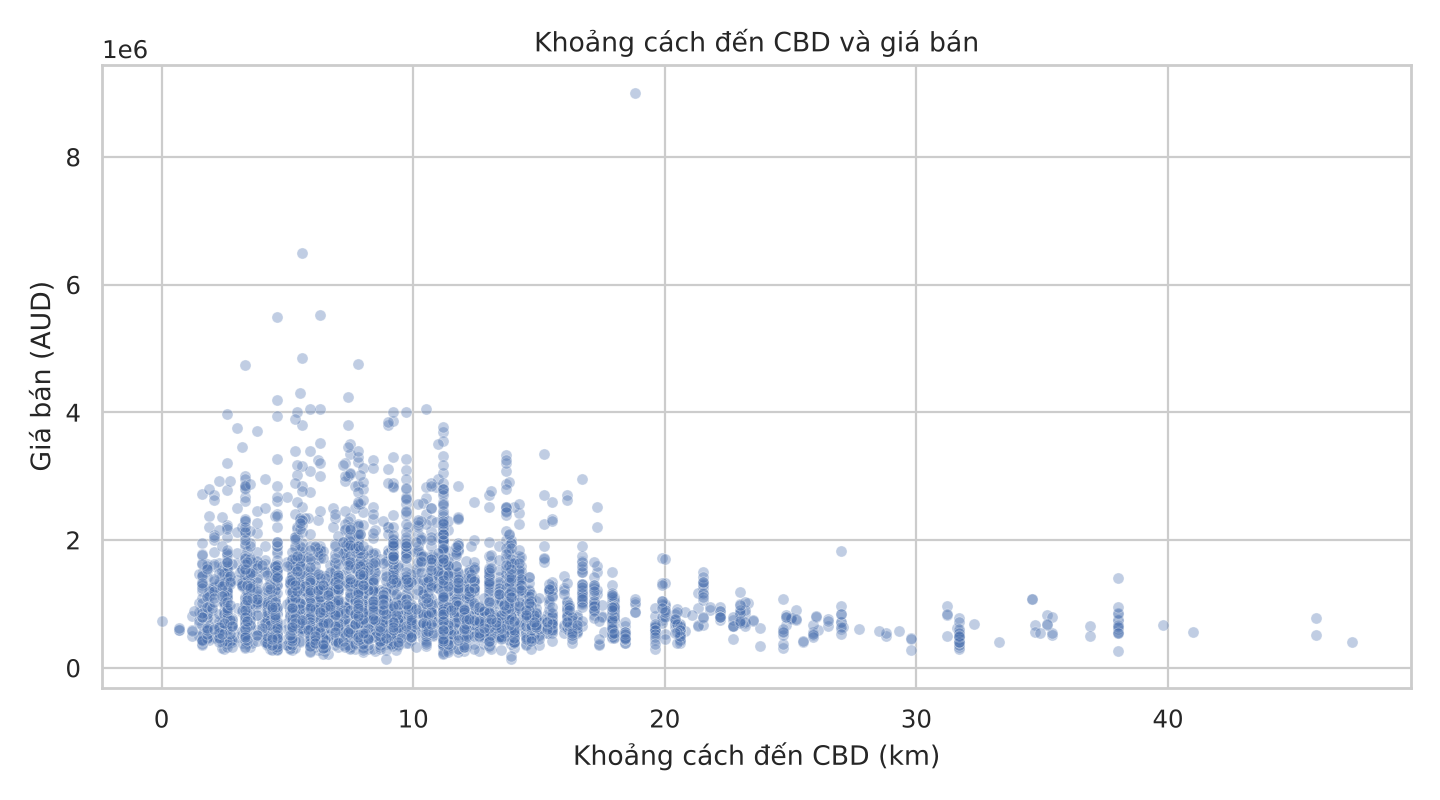
\includegraphics[width=0.72\linewidth]{04_price_vs_distance.png}
\caption{Khoảng cách đến trung tâm (CBD) và giá bán, mẫu ngẫu nhiên 4,000 điểm}\label{fig:distance}
\nguon{\texttt{outputs/04\_price\_vs\_distance.png}; hệ số tương quan: \bs{P07}; tỷ lệ theo khoảng cách: \bs{P09}.}
\end{figure}
Trong 1,007 giao dịch trên 2 triệu AUD, 97.2\% nằm trong 15 km; trong 731 giao dịch ngoài 20 km, 97.9\% dưới 1.5 triệu AUD (\bs{P09}).

\section{Theo thời gian}\label{sec:xuhuong}\label{sec:p7}
\paragraph{Phép 7. Giá theo tháng bán.} Nhóm theo \texttt{SaleMonth} và tính trung vị (\texttt{outputs/price\_by\_sale\_month.csv}). Trừ tháng 1 (2 giao dịch), trung vị dao động quanh 890,000 đến 970,000, trừ tháng 7 thấp rõ rệt (773,500) (\bs{P08}). Điểm trũng này cần đọc thận trọng: ở tháng 7/2017 chỉ 19.3\% giao dịch thuộc Southern Metropolitan (tháng 6: 29.5\%, tháng 8: 30.0\%), nên cơ cấu thiên về vùng rẻ hơn và giá thấp chưa chắc là giá giảm. Theo năm, trung vị gần như đi ngang: 900,000 (2016) và 910,000 (2017 đến 23/09), tăng khoảng 1.1\% (\bs{P08}). Dữ liệu chỉ dài 19 tháng và có khoảng trống nên kết luận chỉ có tính mô tả.
